\documentclass[11pt,a4paper]{article}
\usepackage[utf8]{inputenc}
\usepackage[T1]{fontenc}
\usepackage{geometry}
\usepackage{graphicx}
\usepackage{xcolor}
\usepackage{hyperref}
\usepackage{booktabs}
\usepackage{array}
\usepackage{longtable}
\usepackage{fancyhdr}
\usepackage{enumitem}
\usepackage{titlesec}
\usepackage{amsfonts}
\usepackage{amssymb}
\usepackage{listings}

% Page setup
\geometry{margin=1in}
\pagestyle{fancy}
\fancyhf{}
\fancyhead[L]{A06 - AgentVisa Project Report}
\fancyhead[R]{CISC 691 - Summer 2025}
\fancyfoot[C]{\thepage}

% Colors
\definecolor{primaryblue}{RGB}{44,62,80}
\definecolor{secondaryblue}{RGB}{52,152,219}
\definecolor{successgreen}{RGB}{39,174,96}

% Hyperlink setup
\hypersetup{
    colorlinks=true,
    linkcolor=primaryblue,
    urlcolor=secondaryblue,
    citecolor=primaryblue
}

% Title formatting
\titleformat{\section}
{\Large\bfseries\color{primaryblue}}
{\thesection}{1em}{}[\titlerule]

\titleformat{\subsection}
{\large\bfseries\color{secondaryblue}}
{\thesubsection}{1em}{}

% Custom commands
\newcommand{\greencheck}{\textcolor{successgreen}{\checkmark}}
\newcommand{\tech}[1]{\textbf{#1}}
\newcommand{\code}[1]{\texttt{#1}}

\begin{document}

% Custom title page
\begin{titlepage}
\centering
\vspace*{\fill}

{\Huge\bfseries\color{primaryblue} A06 - AgentVisa Project Report} \\
\vspace{0.8cm}
{\Large AI Assistant for Visa Bulletin Insights} \\
\vspace{0.8cm}
{\large CISC 691 - Foundations of Next-Gen AI} \\

\vspace{2cm}

{\large\textbf{Tien Dinh \& Kenneth Peter Fernandes}} \\
\vspace{0.5cm}
{\large Harrisburg University} \\
{\large Summer 2025} \\

\vspace{1cm}

{\large \today}

\vspace*{\fill}
\end{titlepage}

\vspace{1cm}

\begin{abstract}
\textbf{AgentVisa} is a comprehensive AI-powered assistant for US visa bulletin analysis built as part of CISC 691 - Foundations of Next-Gen AI course assignment. The project demonstrates advanced AI agent development with multi-provider LLM support, containerized microservices architecture, and production-ready cloud deployment capabilities. 

The system integrates five major LLM providers including Google Gemini, OpenAI GPT, Anthropic Claude, Ollama, and HuggingFace Transformers, providing robust fallback mechanisms and flexibility in AI model selection. Built on a microservices architecture using FastAPI and Streamlit, the application processes real visa bulletin data from the US State Department, applying machine learning algorithms for trend analysis and predictive modeling.

The project successfully implements intelligent tool-calling capabilities, enabling the AI agent to automatically select and execute specialized visa analytics functions based on user queries. Comprehensive deployment strategies include local development with Docker Compose, Kubernetes orchestration with Minikube, and production-ready Google Kubernetes Engine deployment with SSL certificates, load balancing, and horizontal pod autoscaling.

This report presents the technical architecture, implementation details, deployment strategies, and performance metrics of a modern AI agent system that validates the practical application of next-generation AI concepts in real-world scenarios. The system includes comprehensive test coverage across unit, integration, and API testing, demonstrating robust software engineering practices alongside cutting-edge AI integration.
\end{abstract}

\newpage
\tableofcontents
\newpage

\section{Executive Summary}

AgentVisa represents a sophisticated implementation of modern AI agent architecture, combining multiple large language model providers with comprehensive visa bulletin analytics. The project successfully demonstrates practical application of AI agent development concepts learned throughout the course, delivering a production-ready system with enterprise-grade infrastructure.

\begin{figure}[h!]
\centering
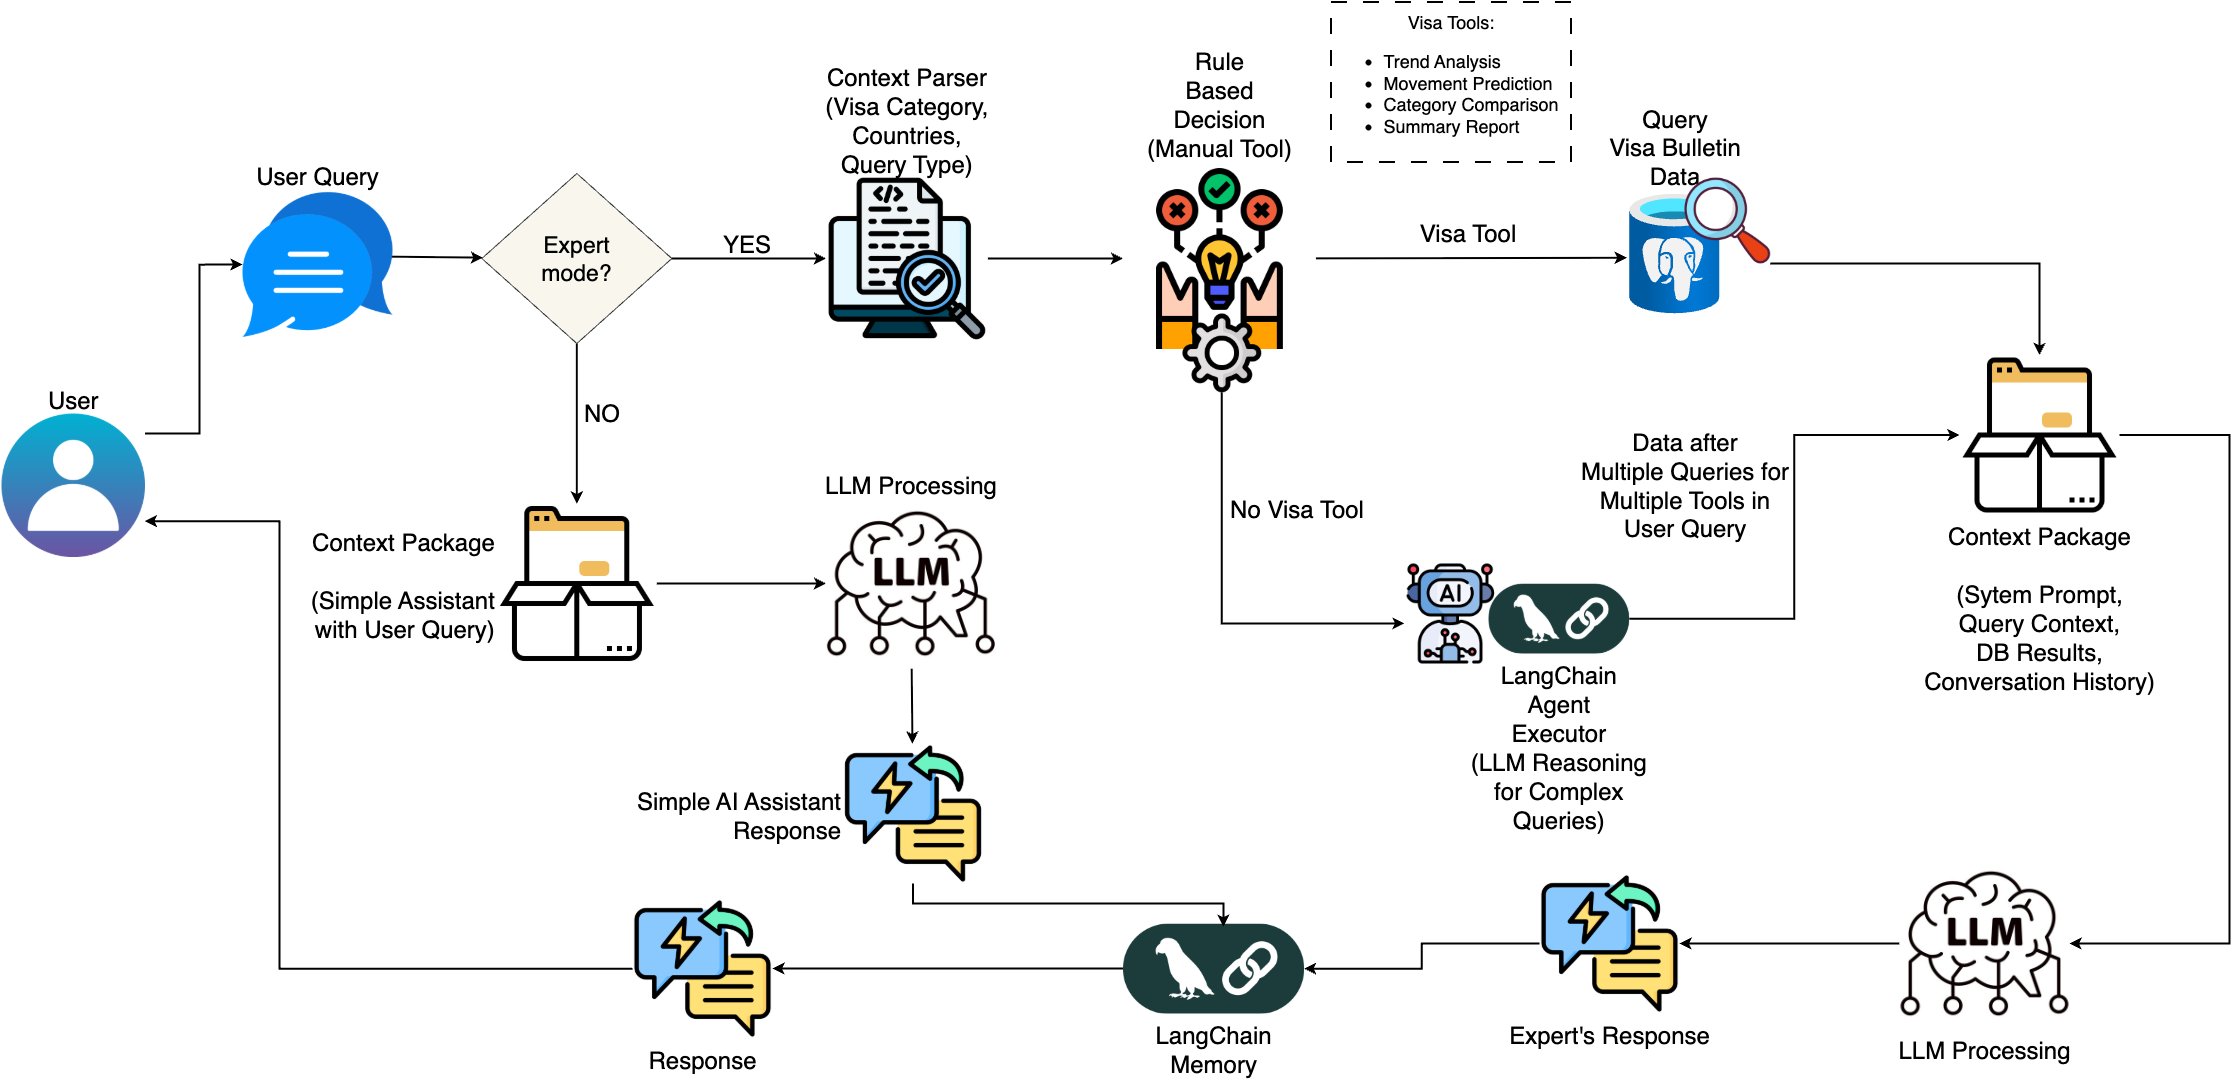
\includegraphics[width=0.8\textwidth]{application-workflow.png}
\caption{AgentVisa Application Workflow - User interactions, AI agent processing, and system responses}
\label{fig:workflow}
\end{figure}

\subsection{Project Overview}
\begin{itemize}[itemsep=0.5em]
    \item \textbf{Project Name:} AgentVisa - AI Assistant for Visa Bulletin Insights
    \item \textbf{Course:} CISC 691 - Foundations of Next-Gen AI (A06: Building the AI Agent of Your Choice)
    \item \textbf{Institution:} Harrisburg University (Summer 2025)
    \item \textbf{Contributors:} Tien Dinh, Kenneth Peter Fernandes
    \item \textbf{Repository:} \url{https://github.com/kenneth-fernandes/cisc691-a06}
    \item \textbf{Testing:} Comprehensive test suite with unit, integration, and API tests
\end{itemize}

\newpage
\section{System Overview \& Architecture}

\subsection{About AgentVisa}
AgentVisa is a containerized AI assistant with REST API backend that provides intelligent US visa bulletin analysis and multi-provider LLM chat capabilities. The system demonstrates advanced AI agent development with modern microservices architecture and production-ready cloud deployment capabilities.

\subsection{Core System Architecture}
Enterprise-ready microservices design with 4 containerized services:

\begin{itemize}[itemsep=0.3em]
    \item \textbf{Web Service:} Streamlit frontend for interactive user interface (Port 8501)
    \item \textbf{API Service:} FastAPI backend for REST API processing (Port 8000)
    \item \textbf{PostgreSQL Database:} Primary data storage with JSONB support (Port 5432)
    \item \textbf{Redis Cache:} High-performance caching layer (Port 6379)
\end{itemize}

\subsection{Dual Operating Modes}
AgentVisa provides two distinct interaction modes:
\begin{itemize}[itemsep=0.3em]
    \item \textbf{General Chat Mode:} Standard AI assistant capabilities for general queries and conversations
    \item \textbf{Visa Expert Mode:} Specialized U.S. visa bulletin analysis with integrated analytics tools and historical data access
\end{itemize}

\newpage
\section{Core Features \& Capabilities}

\subsection{Multi-Provider AI Agent System}
The system supports multiple LLM providers with intelligent fallback mechanisms:

\begin{itemize}[itemsep=0.3em]
    \item \tech{Google Gemini (gemini-1.5-flash)} - Free tier, fast responses, and cost-effective (Primary)
    \item \tech{Ollama (llama3.2)} - Offline processing, no API costs, and complete data privacy (Local)
    \item \tech{OpenAI GPT (gpt-4o)} - Excellent for complex reasoning, nuanced immigration logic, and high reliability
    \item \tech{Anthropic Claude (claude-3-5-sonnet)} - Long-context processing, trend analysis, and strong safety guarantees
    \item \tech{HuggingFace Transformers} (Local, Free) - Community models for specialized tasks
\end{itemize}

\subsection{Visa Bulletin Analytics Engine}
Comprehensive analytics capabilities for US visa bulletin data:

\begin{itemize}[itemsep=0.3em]
    \item \textbf{Complete Category Support:} EB-1 through EB-5, F1 through F4
    \item \textbf{Country Analysis:} India, China, Mexico, Philippines, Worldwide
    \item \textbf{ML-Powered Predictions:} Random Forest \& Logistic Regression models
    \item \textbf{Historical Data:} 2020-present with automated monthly updates
    \item \textbf{Interactive Dashboards:} Charts and visualizations
\end{itemize}

\subsection{Data Processing Pipeline}
Automated visa bulletin data collection and processing:

\begin{itemize}[itemsep=0.3em]
    \item \textbf{Web Scraping:} BeautifulSoup4-based HTML parsing from travel.state.gov
    \item \textbf{Data Validation:} Multi-stage quality assurance and verification
    \item \textbf{Historical Analysis:} Trend analysis from 2020-present
    \item \textbf{Predictive Modeling:} ML-powered forecast algorithms
\end{itemize}

\begin{figure}[h!]
\centering
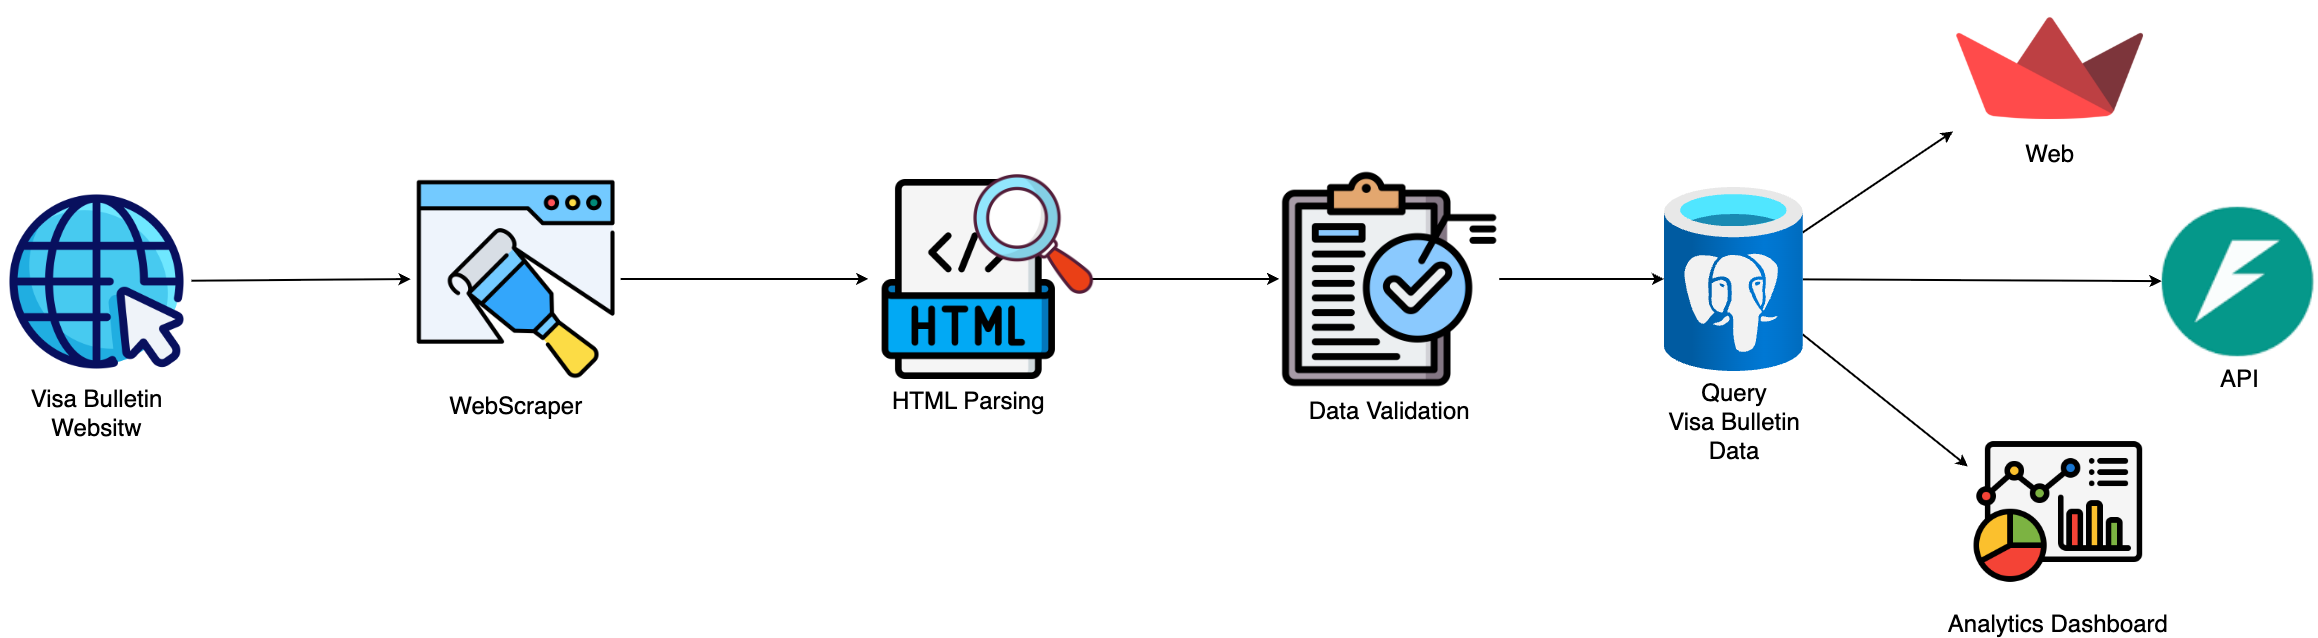
\includegraphics[width=0.9\textwidth]{visa-data-fetching.png}
\caption{Visa Data Fetching Pipeline - Automated data collection from US State Department through validation to database storage}
\label{fig:data-pipeline}
\end{figure}

\newpage
\section{Technical Implementation}

\subsection{Core Components}

\subsubsection{AI Agent Core (\code{src/agent/core.py})}
The central AI agent implementation featuring:
\begin{itemize}[itemsep=0.2em]
    \item Multi-provider LLM integration with fallback support
    \item Conversation memory management
    \item Tool-calling capabilities for visa analytics
    \item Context-aware response generation
\end{itemize}

\subsubsection{FastAPI Backend (\code{src/api/main.py})}
RESTful API service providing:
\begin{itemize}[itemsep=0.2em]
    \item RESTful API endpoints for agent interactions
    \item CORS middleware for cross-origin requests
    \item Global exception handling
    \item Health check endpoints
\end{itemize}

\subsubsection{Data Processing Pipeline}
Automated data collection and processing:
\begin{itemize}[itemsep=0.2em]
    \item Automated visa bulletin scraping from travel.state.gov
    \item Multi-stage data validation and quality assurance
    \item Historical data collection and storage
    \item ML model training and prediction
\end{itemize}

\subsection{Deployment Options}

\begin{table}[h!]
\centering
\begin{tabular}{@{}lllll@{}}
\toprule
\textbf{Method} & \textbf{Use Case} & \textbf{Setup Time} & \textbf{Cost} & \textbf{Security} \\
\midrule
GKE Production & Production deployment & 12-20 min & \textasciitilde\$143/month & Enterprise \\
Minikube Local & Development/testing & 5-10 min & Free & Basic \\
Docker Compose & Quick testing & 2-5 min & Free & None \\
\bottomrule
\end{tabular}
\caption{Deployment Options Comparison}
\end{table}

\begin{figure}[h!]
\centering
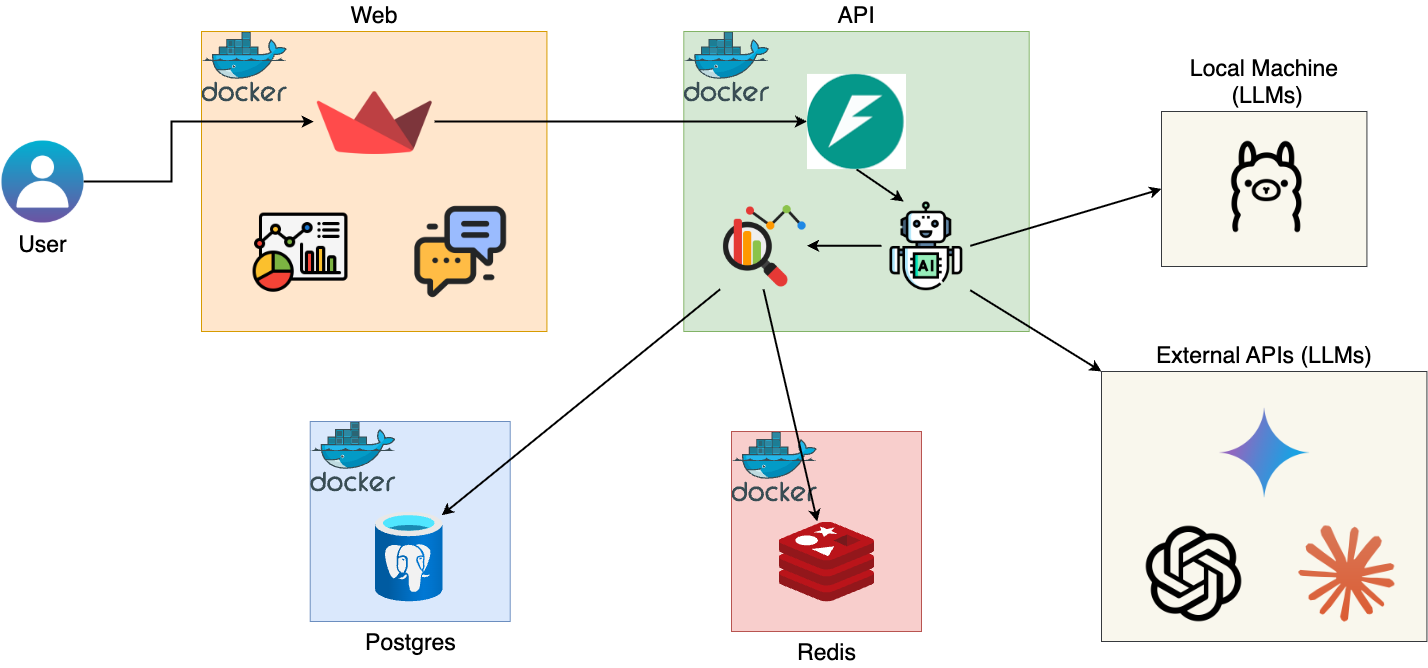
\includegraphics[width=0.8\textwidth]{local-docker-deployment.png}
\caption{Local Docker Deployment - Microservices architecture for development}
\label{fig:docker}
\end{figure}

\begin{figure}[h!]
\centering
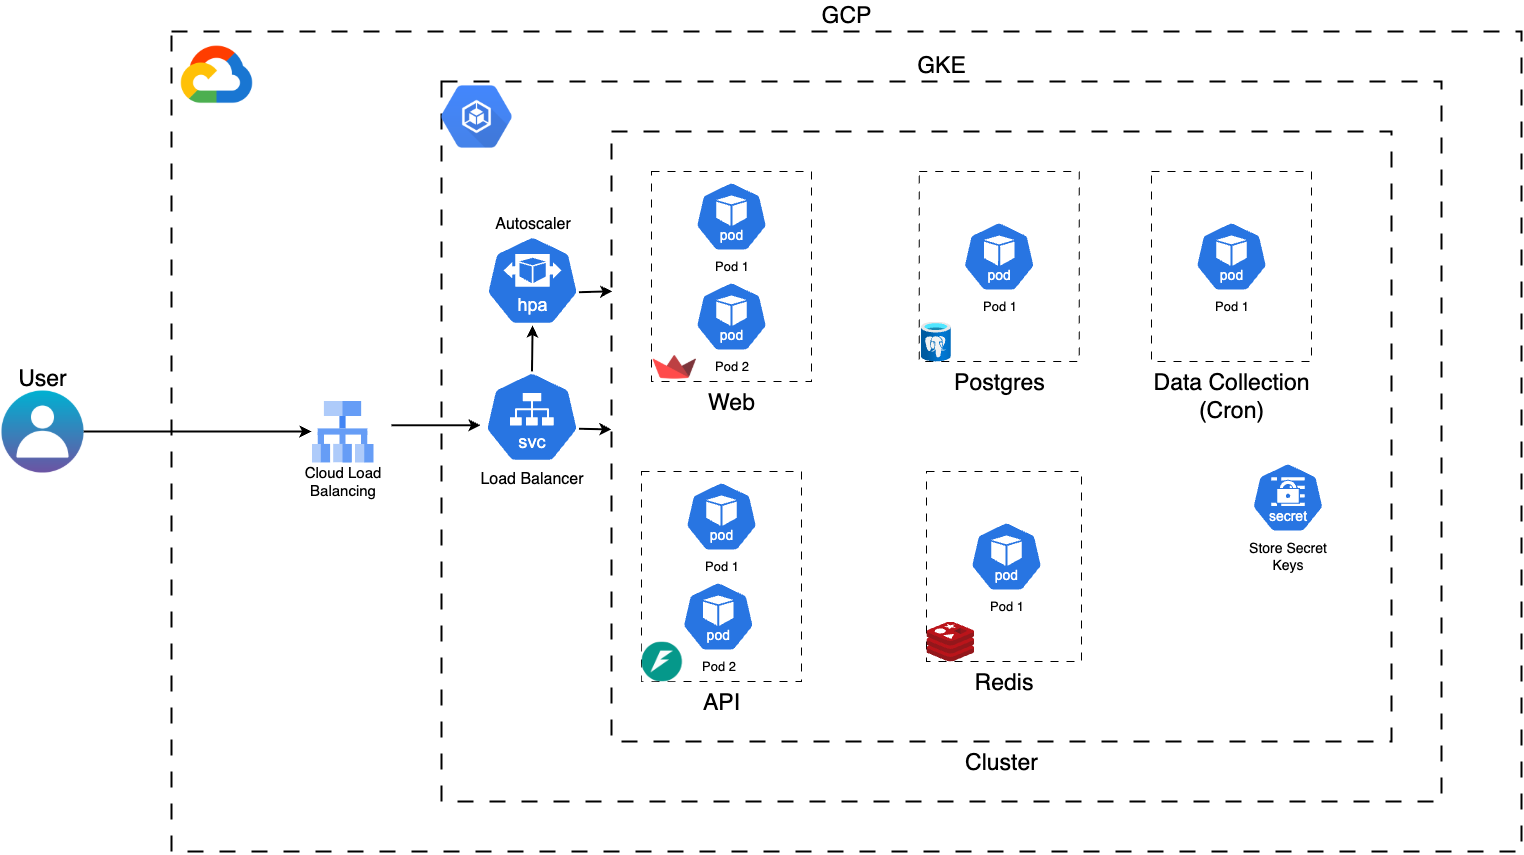
\includegraphics[width=0.8\textwidth]{gke-cloud-architecture.png}
\caption{GKE Cloud Architecture - Production deployment with scaling}
\label{fig:gke}
\end{figure}

\subsection{Infrastructure Features}
\begin{itemize}[itemsep=0.3em]
    \item \textbf{Kubernetes Orchestration:} Full k8s deployment with autoscaling
    \item \textbf{SSL/TLS Security:} Google-managed certificates
    \item \textbf{Load Balancing:} Production-grade traffic distribution
    \item \textbf{Horizontal Pod Autoscaling:} Automatic resource scaling
    \item \textbf{Terraform Automation:} Infrastructure as Code
\end{itemize}

\newpage
\section{Key Technologies \& Dependencies}

\subsection{AI/ML Stack}
\begin{itemize}[itemsep=0.2em]
    \item \tech{LangChain Framework:} Agent orchestration and tool integration
    \item \tech{Scikit-learn:} ML models for visa prediction
    \item \tech{Pandas/NumPy:} Data processing and analysis
\end{itemize}

\subsection{Web Framework}
\begin{itemize}[itemsep=0.2em]
    \item \tech{FastAPI:} Modern async web framework
    \item \tech{Streamlit:} Interactive frontend interface
    \item \tech{Uvicorn:} ASGI server implementation
\end{itemize}

\subsection{Database \& Caching}
\begin{itemize}[itemsep=0.2em]
    \item \tech{PostgreSQL:} Primary database with JSONB support
    \item \tech{Redis:} High-performance caching layer
\end{itemize}

\subsection{DevOps \& Testing}
\begin{itemize}[itemsep=0.2em]
    \item \tech{Docker/Docker Compose:} Containerization
    \item \tech{Kubernetes:} Container orchestration
    \item \tech{Pytest:} Comprehensive testing suite
    \item \tech{GitHub Actions:} CI/CD pipeline
\end{itemize}

\newpage
\section{Deployment \& Operations}

\subsection{Deployment Architecture Overview}
AgentVisa supports multiple deployment strategies optimized for different use cases:

\begin{table}[h!]
\centering
\begin{tabular}{@{}lllll@{}}
\toprule
\textbf{Method} & \textbf{Use Case} & \textbf{Setup Time} & \textbf{Cost} & \textbf{Security} \\
\midrule
GKE Production & Production deployment & 12-20 min & \textasciitilde\$143/month & Enterprise \\
Minikube Local & Development/testing & 5-10 min & Free & Basic \\
Docker Compose & Quick testing & 2-5 min & Free & None \\
\bottomrule
\end{tabular}
\caption{Deployment Options Comparison}
\end{table}

\begin{figure}[h!]
\centering
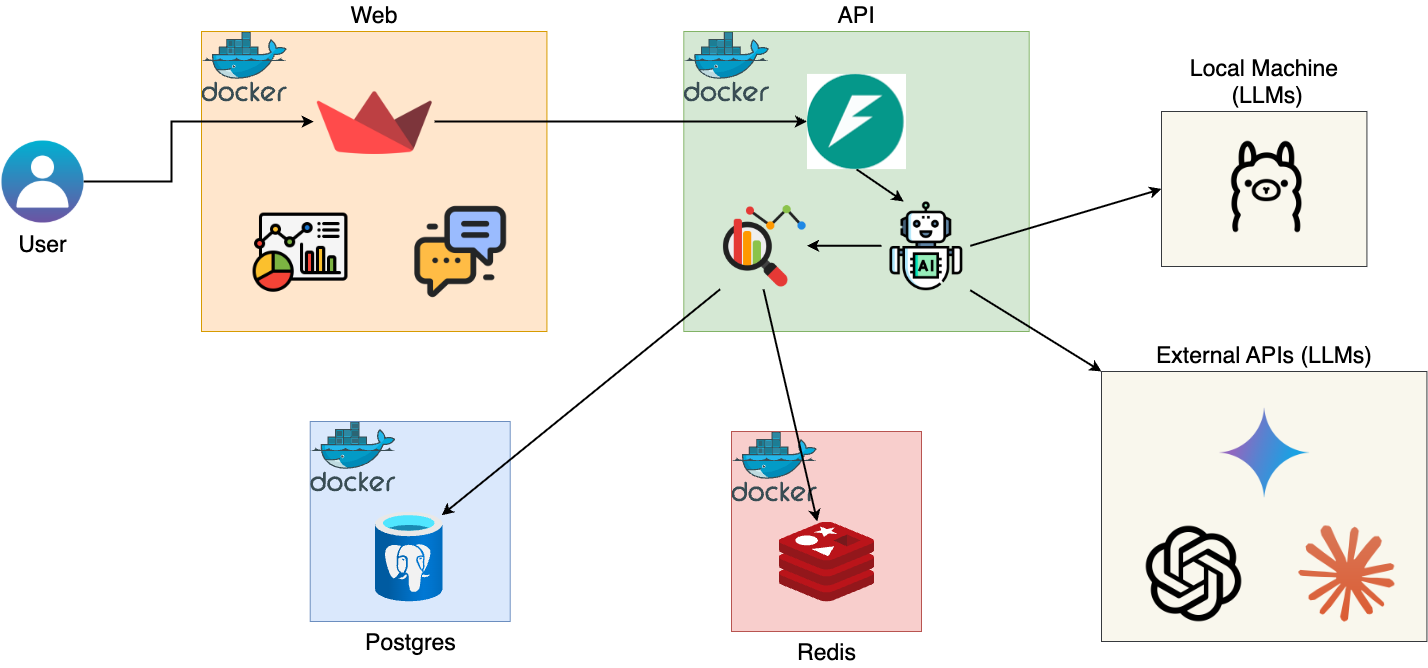
\includegraphics[width=0.8\textwidth]{local-docker-deployment.png}
\caption{Local Docker Deployment - Microservices architecture for development}
\label{fig:docker}
\end{figure}

\begin{figure}[h!]
\centering
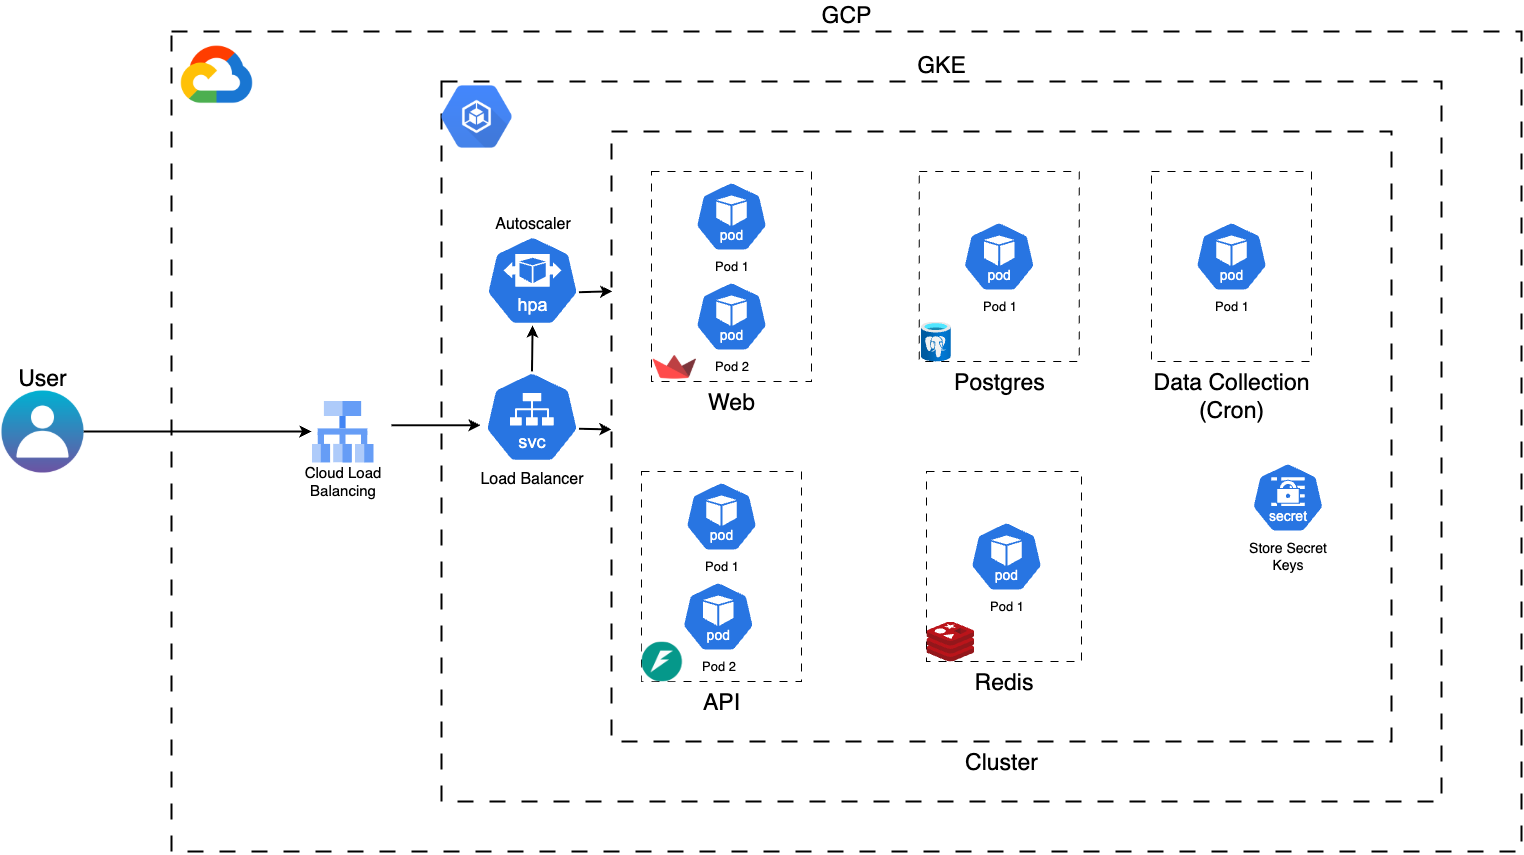
\includegraphics[width=0.8\textwidth]{gke-cloud-architecture.png}
\caption{GKE Cloud Architecture - Production deployment with scaling}
\label{fig:gke}
\end{figure}

\subsection{Cloud Infrastructure (GKE)}
Production deployment on Google Kubernetes Engine features:
\begin{itemize}[itemsep=0.3em]
    \item \textbf{Google Cloud Platform:} Primary cloud provider with integrated services
    \item \textbf{Kubernetes Engine:} Managed container orchestration with autoscaling
    \item \textbf{Terraform Automation:} Infrastructure as Code for consistent deployments
    \item \textbf{Kubernetes Secrets:} Secure API key and credential management
    \item \textbf{Load Balancing:} Production-grade traffic distribution with health checks
    \item \textbf{SSL/TLS Security:} Google-managed certificates with automatic renewal
\end{itemize}

\subsection{Local Development Environment}
Developer-friendly local setup options:
\begin{itemize}[itemsep=0.3em]
    \item \textbf{Minikube:} Local Kubernetes environment for testing
    \item \textbf{Docker Compose:} Simplified multi-container orchestration
    \item \textbf{Hot Reload:} Development-friendly configuration with live updates
    \item \textbf{Resource Optimization:} Efficient resource usage for local development
\end{itemize}

\newpage
\section{Development Highlights}

\subsection{Advanced System Features}
\begin{enumerate}[itemsep=0.3em]
    \item \textbf{Intelligent Tool Integration:} Automatic tool selection based on query context and user intent
    \item \textbf{Multi-Provider Fallback:} Seamless switching between LLM providers with graceful degradation
    \item \textbf{Production Monitoring:} Comprehensive health checks, logging, and observability with K9s dashboard
    \item \textbf{Cost Optimization:} Efficient resource utilization and automated scaling (\textasciitilde\$143/month for cloud)
\end{enumerate}

\newpage
\section{Quality Assurance}

\subsection{Testing Strategy}
The project implements comprehensive testing across multiple dimensions:
\begin{itemize}[itemsep=0.3em]
    \item \textbf{Unit Tests:} Individual component testing
    \item \textbf{Integration Tests:} End-to-end workflow validation
    \item \textbf{API Tests:} REST endpoint functionality
    \item \textbf{Cache Tests:} Redis performance and fallback
    \item \textbf{Testing Focus:} Core APIs and critical functionality covered
\end{itemize}

\subsection{Development Best Practices}
\begin{itemize}[itemsep=0.3em]
    \item \textbf{Clean Architecture:} Layered design with separation of concerns
    \item \textbf{Factory Patterns:} Flexible agent creation and configuration
    \item \textbf{Environment Configuration:} Secure secret management
    \item \textbf{Documentation:} Comprehensive markdown documentation
\end{itemize}


\newpage
\section{Project Success Metrics}

\subsection{Technical Achievements}
\begin{itemize}[itemsep=0.3em]
    \item[\greencheck] Multi-provider AI agent successfully implemented
    \item[\greencheck] Production-ready microservices architecture
    \item[\greencheck] Comprehensive visa analytics with ML predictions
    \item[\greencheck] Full containerization and k8s deployment
    \item[\greencheck] Automated CI/CD pipeline with testing
\end{itemize}

\subsection{Learning Objectives Met}
\begin{itemize}[itemsep=0.3em]
    \item[\greencheck] Modern AI framework integration (LangChain)
    \item[\greencheck] Multiple LLM provider support and flexibility
    \item[\greencheck] Modular and extensible architecture design
    \item[\greencheck] Practical AI integration skills demonstration
\end{itemize}

\newpage
\section{Future Enhancements \& Recommendations}

\begin{enumerate}[itemsep=0.4em]
    \item \textbf{Enhanced ML Models:} Implement deep learning for improved predictions
    \item \textbf{Real-time Updates:} WebSocket integration for live data streaming
    \item \textbf{Advanced Analytics:} More sophisticated trend analysis and reporting
    \item \textbf{Mobile Support:} React Native or Progressive Web App
    \item \textbf{API Rate Limiting:} Enhanced security and resource protection
\end{enumerate}

\newpage
\section{API Architecture \& Endpoints}

The AgentVisa system exposes a comprehensive REST API organized into three main categories:

\subsection{Core Agent Endpoints}
\begin{itemize}[itemsep=0.3em]
    \item \code{POST /api/agent/chat} - Send messages to AI agent with dual mode support
    \item \code{GET /api/agent/conversation/\{id\}} - Retrieve chat history and conversation state
    \item \code{GET /api/agent/providers} - List available LLM providers and their status
\end{itemize}

\subsection{Visa Analytics Endpoints}
\begin{itemize}[itemsep=0.3em]
    \item \code{POST /api/analytics/trends} - Analyze historical visa bulletin trends
    \item \code{POST /api/analytics/predictions} - Generate ML-powered forecasting predictions
    \item \code{GET /api/analytics/historical} - Access historical visa bulletin data
\end{itemize}

\subsection{Data Access Endpoints}
\begin{itemize}[itemsep=0.3em]
    \item \code{GET /api/analytics/categories} - Retrieve supported visa categories (EB-1 to EB-5, F1 to F4)
    \item \code{GET /api/analytics/countries} - List supported countries for analysis
    \item \code{GET /api/analytics/bulletins} - Access available bulletin dates and metadata
\end{itemize}

\newpage
\section{Challenges \& Technical Learnings}

The development process provided valuable insights into modern AI system deployment and integration challenges:

\subsection{Communication Architecture Decisions}
\begin{itemize}[itemsep=0.3em]
    \item \textbf{WebSocket Integration Issues:} Initial WebSocket implementation with Streamlit proved unstable, leading to adoption of reliable HTTP-based communication for better compatibility and stability
    \item \textbf{Solution:} Implemented robust REST API communication patterns with proper error handling and timeout management
\end{itemize}

\subsection{Cloud Deployment Challenges}
\begin{itemize}[itemsep=0.3em]
    \item \textbf{Ollama on GKE Limitations:} CPU constraints and lack of GPU support made llama3 1B/3B models unstable without custom high-resource nodes
    \item \textbf{Autoscaling Delays:} Resource constraints occurred when autoscaler delayed node provisioning during experimental pod additions
    \item \textbf{Data Population:} Initial visa data insertion issues resolved through Kubernetes cron job implementation for automated data population
\end{itemize}

\subsection{Local Development Optimizations}
\begin{itemize}[itemsep=0.3em]
    \item \textbf{M2 Air Performance:} Docker performance limitations due to resource constraints and lack of GPU support necessitated use of compact models like LLaMA 3.2 1B
    \item \textbf{Solution:} Optimized local development workflow with efficient model selection and resource management
\end{itemize}

\subsection{Development Tools \& AI Integration}
\begin{itemize}[itemsep=0.3em]
    \item \textbf{AI-Enhanced Development:} Extensive use of VS Code with GitHub Copilot and Claude for AI-enhanced coding, auto-suggestions, and intelligent code reviews
    \item \textbf{Collaboration:} Project developed through intensive brainstorming sessions with Claude AI and ChatGPT, demonstrating effective human-AI collaboration
\end{itemize}

\newpage
\section{Conclusion}

AgentVisa successfully demonstrates the practical application of modern AI agent development concepts, combining multiple cutting-edge technologies into a cohesive, production-ready system. The project showcases technical proficiency in AI/ML, cloud infrastructure, and software engineering best practices while delivering genuine value through intelligent visa bulletin analysis.

The comprehensive architecture, from local development to cloud deployment, reflects industry-standard practices and positions the project as a strong foundation for further AI agent development endeavors. The successful integration of multiple LLM providers, sophisticated data processing pipelines, and enterprise-grade deployment infrastructure validates the learning objectives of the CISC 691 course.

As demonstrated through the visual architecture diagrams (Figures \ref{fig:workflow}, \ref{fig:docker}, \ref{fig:gke}, and \ref{fig:data-pipeline}), the system provides a complete end-to-end solution for AI-powered visa bulletin analysis, from data collection through user interaction and intelligent response generation.

\vspace{1cm}

\hrule

\vspace{0.5cm}

\begin{center}
\textit{Generated on: \today} \\
\textit{Project: AgentVisa - AI Assistant for Visa Bulletin Insights} \\
\textit{Course: CISC 691 - Foundations of Next-Gen AI}
\end{center}

\end{document}